\documentclass[parskip=half]{scrartcl}

\usepackage[paperheight=3.5in, paperwidth=2.5in, margin=0.25in]{geometry}

\usepackage{fontspec}
\usepackage{enumitem}
\usepackage{caption}
\setmainfont{URWClassico}
\usepackage{tikz}

\definecolor{eruption_purple}{HTML}{513c3c}
\definecolor{eruption_pink}{HTML}{ff7280}

\setkomafont{section}{\setmainfont{LondrinaSolid}\Large\color{eruption_purple}}
\setkomafont{subsection}{\setmainfont{LondrinaSolid}\large\color{eruption_purple}}
\setkomafont{subsubsection}{\setmainfont{LondrinaSolid}\normalsize\color{eruption_purple}}

% Adjust spacing before and after section headings
\RedeclareSectionCommand[
  runin=false,
  beforeskip=0.5\baselineskip,
  afterskip=-0.0\baselineskip
]{section}

% Adjust spacing before and after subsection headings
\RedeclareSectionCommand[
  runin=false,
  beforeskip=0.5\baselineskip,
  afterskip=-0.0\baselineskip
]{subsection}

% Adjust spacing before and after subsubsection headings
\RedeclareSectionCommand[
  runin=false,
  beforeskip=0.5\baselineskip,
  afterskip=-0.0\baselineskip
]{subsubsection}

\tikzset{ring/.pic={
\pgfmathsetseed{#1} 

\foreach \i/\j in {0,72,...,359}
 \node[gray, fill=black, minimum width=3.5mm, minimum height=3.5mm, rotate=180*rand] at (\i:5mm) {};
 
\foreach \i/\j in {36,108,...,359}
 \node[gray, fill=black, minimum width=3.5mm, minimum height=3.5mm, rotate=180*rand] at (\i:7.5mm) {};

 \node[draw, gray, fill=white, minimum width=3.5mm, minimum height=3.5mm, rotate=180*rand] at (0,0) {};

 \draw[ultra thick, brown] plot[smooth cycle,variable=\t,samples at={0,45,...,315}] (\t:rr);
}
}


\usepackage{hyperref}

%\pagecolor{eruption_pink}
\begin{document}
\color{eruption_purple}
{
\enlargethispage{1.0\baselineskip}
\begin{center}
\setmainfont[Scale=1.0]{Earthquake MF} \Huge
ERUPTION

\setmainfont{URWClassico} \scriptsize
A dexterity game for 2\textendash{}6 players

\vfill

\includegraphics[width=2.0in]{Images/one_volcano.png}

\vfill

\setmainfont{URWClassico}
\normalsize
Designed by Michael Purcell
\end{center}
}

\newpage
\raggedright
\setmainfont{URWClassico} \small
\section*{Overview}
Eruption is a dexterity game for 2\textendash{}6 players. It can be played in about fifteen minutes and is intended for players who are at least twelve years old.

\section*{Components}
\begin{itemize}[leftmargin=*]
\item 175 wooden cubes (8mm)
\begin{itemize}[leftmargin=*]
\item 120 lava cubes (40 each of red, orange, and yellow)
\item 50 black cubes
\item 5 white cubes
\end{itemize}
\item 5 rubber bands (size \#31)
\end{itemize}

\newpage

\section*{Set Up}
\begin{enumerate}[leftmargin=*]
\item Choose one player to go first.

\item Each other player should place a rubber band in the middle of the play area.

\item Place ten black cubes and one white cube inside the ring formed by each rubber band.
\end{enumerate}

\vfill

\begin{figure}[hb]
\centering
%\begin{center}
\scalebox{0.55}{
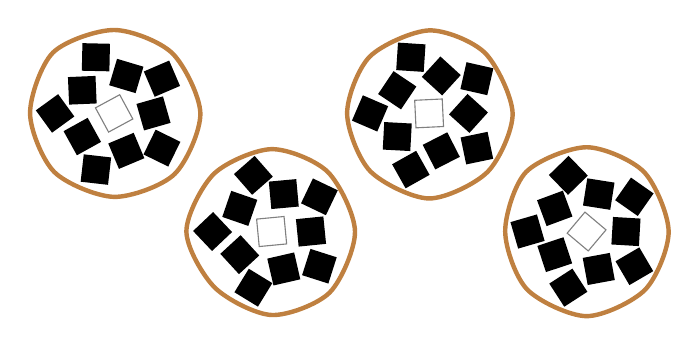
\begin{tikzpicture}[declare function={rr=1.0*(1+0.1*rnd);}]
\pic at (0,0) {ring={3}};

\pic at (6cm, -1.5cm) {ring={5}};

\pic at (2cm, -1.5cm) {ring={18}};

\pic at (4, 0cm) {ring={9}};
\end{tikzpicture}
}
%\end{center}
\caption*{{\scriptsize Setup for a five-player game.}}
\end{figure}
\newpage
\section*{Gameplay}
On your turn, place a lava cube into one of the rings.
\begin{itemize}[leftmargin=*]
\item You must place your cube so that it is touching a white cube.
\item You may only use one hand at a time while placing your cube.
\end{itemize}

If any cubes fall out of the ring during your turn, you and the ring are eliminated from the game.

You win if all of your opponents have been eliminated.

\vfill
%\hrulefill

\scriptsize
\textbf{Contact}: \href{mailto:ttkttkt@gmail.com}{ttkttkt@gmail.com}\\
\textbf{License}: This work is licensed under a\\\phantom{\textbf{License}: }``CC BY-SA 4.0'' license.%\raggedright\doclicenseText
 
\end{document}